%!TEX root = Slic3r-Manual.tex

\section{Largeur d'Extrusion} % (fold)
\label{sec:extrusion_width}
\index{extrusion width}
\index{largeur d'extrusion}

\begin{figure}[H]
\centering
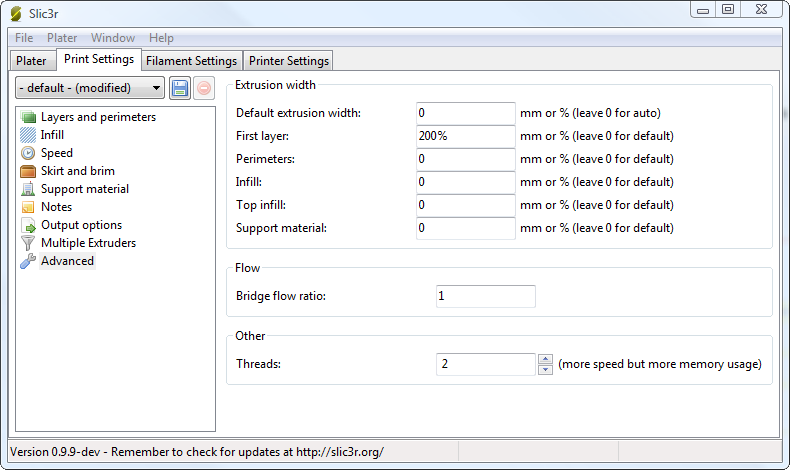
\includegraphics[keepaspectratio=true,width=1\textwidth]{expertmode/advanced_extrusion_widths_options.png}
\caption{Paramètres de largeur d'Extrusion.}
\label{fig:advanced_extrusion_widths_options}
\end{figure}

Une des raisons de la modification de la largeur de l'extrusion a déjà été examinée: l'augmentation de la largeur d'extrusion de la première couche dans le but d'améliorer l'adhesion au lit. (voir p.\pageref{par:wider_extrusion_width}).  Il ya quelques autres cas où il peut être bénéfique de modifier la largeur d'extrusion.
\begin{itemize}
    \item \texttt{Perimeter} (Périmètre) - Une valeur plus faible produira des extrusions minces qui à leurs tour produiront des surfaces plus précise.
    \item \texttt{Infill} (Remplissage) et \texttt{Solid Infill} (Remplissage solide) - Une extrusion épaisse pour le remplissage produira des impressions plus rapides et des pièces plus solides.
    \item \texttt{Top infill} (Remplissage suppérieur) - Une extrusion fine, améliorera la finition de la surface et assurera que es coins soit bien remplis.
    \item \texttt{Support material} (Matière de Support) - Comme avec les options de remplissage, une extrusion épaisse permettra de réduire le temps d'impression.
\end{itemize}

Il est important de se rappeler que, si la largeur de l'extrusion est exprimée en pourcentage, elle se calcule à partir de la propriété \texttt{Layer height} (Hauteur de couche), et non du paramètre \texttt{Default extrusion width} (Largeur d'extrusion par défaut).

% section extrusion_width (end)